
\documentclass[aspectratio=169]{beamer}
\usetheme{Madrid}
\usecolortheme{default}
\setbeamertemplate{navigation symbols}{}
\setbeamertemplate{footline}{%
  \leavevmode%
  \hbox{%
    \begin{beamercolorbox}[wd=.74\paperwidth,ht=2.6ex,dp=1ex,leftskip=1em]{author in head/foot}%
      \insertshorttitle\hspace{1em}|\hspace{1em}\insertshortauthor
    \end{beamercolorbox}%
    \begin{beamercolorbox}[wd=.26\paperwidth,ht=2.6ex,dp=1ex,rightskip=1em plus 1fil]{date in head/foot}%
      \hfill\insertframenumber/\inserttotalframenumber
    \end{beamercolorbox}%
  }%
  \vskip0pt%
}
\usepackage[utf8]{inputenc}
\usepackage{booktabs}
\usepackage{graphicx}
\usepackage{amsmath}
\usepackage{xcolor}
\graphicspath{{results/plots/}{../results/plots/}}

\title[AlgoBench]{AlgoBench}
\subtitle{Algorithm Benchmarking \& Profiling Suite}
\author{SSL Project Team}
\institute{Department of Computer Science and Engineering\\Indian Institute of Technology Dharwad}
\date{November 2026}

\begin{document}

\begin{frame}
  \titlepage
  \vspace{-0.5em}
  \centering
  \small CS25BT005 \quad MC25BT022 \quad CS25BT031 \quad CS25BT041 \quad CS25BT051
\end{frame}

\begin{frame}{Problem and Motivation}
  \begin{itemize}
    \item Complexity analysis explains growth trends, but not every practical implementation difference.
    \item Observed performance depends on input size, input distribution, implementation, and memory allocation.
    \item Repeated experiments are needed to compare algorithms under controlled, reproducible conditions.
  \end{itemize}
  \vspace{0.8em}
  \begin{block}{Our goal}
    Build one environment to configure experiments, measure algorithms, inspect bottlenecks, and compare results.
  \end{block}
\end{frame}

\begin{frame}{What AlgoBench Does}
  \begin{enumerate}
    \item Select a domain and algorithms.
    \item Generate deterministic input datasets from a chosen seed.
    \item Execute warm-up and repeated timing trials.
    \item Measure peak additional Python memory separately.
    \item Optionally inspect function costs with cProfile/pstats.
    \item Save CSV results and visualize scaling with charts/GNUplot.
  \end{enumerate}
\end{frame}

\begin{frame}{Five Algorithm Domains}
  \small
  \begin{tabular}{p{0.22\textwidth}p{0.68\textwidth}}
    \toprule
    \textbf{Domain} & \textbf{Implementations}\\
    \midrule
    Sorting & Quick, Merge, Heap, Insertion Sort\\
    Searching & Linear, Binary, Hash Table Lookup\\
    Graph & Dijkstra, Bellman--Ford, BFS\\
    Dynamic Programming & LCS and 0/1 Knapsack (memoization/tabulation)\\
    Matrix & Standard and Strassen Multiplication\\
    \bottomrule
  \end{tabular}
  \vspace{0.8em}
  \begin{block}{Total}
    16 registered algorithm implementations.
  \end{block}
\end{frame}

\begin{frame}{System Architecture}
  \small
  \begin{block}{1. Streamlit Dashboard}
    Configure experiments, launch runs, compare results, inspect profiles, browse history.
  \end{block}
  \vspace{-0.75em}
  \begin{center}\scriptsize$\Downarrow$\end{center}
  \vspace{-0.85em}
  \begin{block}{2. Algorithm Registry + Dataset Generators}
    Resolve the selected callable and prepare its reproducible input arguments.
  \end{block}
  \vspace{-0.75em}
  \begin{center}\scriptsize$\Downarrow$\end{center}
  \vspace{-0.85em}
  \begin{block}{3. Generic Benchmark Engine}
    Repeated timing, separate memory measurement, optional cProfile, CSV persistence.
  \end{block}
  \vspace{-0.75em}
  \begin{center}\scriptsize$\Downarrow$\end{center}
  \vspace{-0.85em}
  \begin{block}{4. Visualization and History}
    Dashboard comparison charts, GNUplot runtime/memory plots, saved experiment history.
  \end{block}
\end{frame}

\begin{frame}{Measurement Methodology}
  \begin{itemize}
    \item Runtime: \texttt{time.perf\_counter()}, warm-up, repeated trials.
    \item Statistics: average, median, min, max, standard deviation.
    \item Memory: separate \texttt{tracemalloc} run; peak additional traced memory in KiB.
    \item Profiling: separate \texttt{cProfile}/\texttt{pstats} run; timing is not contaminated by profiler overhead.
    \item Reproducibility: dataset generators accept a random seed.
  \end{itemize}
  \begin{alertblock}{Fair comparison}
    Dataset preparation and input copying are excluded from the timed algorithm call and documented in the result notes.
  \end{alertblock}
\end{frame}

\begin{frame}{Testing and Validation}
  \begin{itemize}
    \item Algorithm correctness and input-validation tests.
    \item Reproducibility tests for graph, string, and matrix generators.
    \item Benchmark timer, memory, profiler, CSV, and GNUplot data tests.
    \item Integration smoke tests execute all 16 registered algorithms through the common engine.
  \end{itemize}
  \vspace{0.5em}
  \begin{block}{Integration test result}
    158 pytest cases passed, plus 64 subtests, in the integration environment.
  \end{block}
  \small Streamlit was run locally; all five domains completed and GNUplot rendered runtime and memory plots.
\end{frame}


\begin{frame}{Measured Results: Sorting and Searching}
  \small
  \begin{columns}[T,onlytextwidth]
    \column{0.50\textwidth}
      \centering\textbf{Sorting: runtime}
      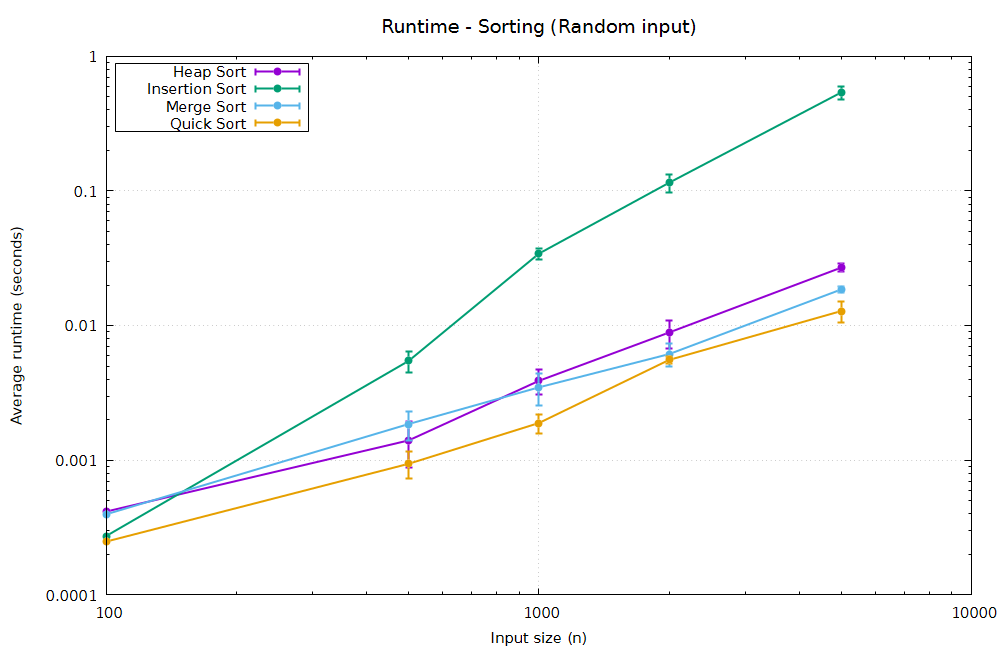
\includegraphics[width=\linewidth,height=0.43\textheight,keepaspectratio]{Sorting_Random_runtime.png}
      \scriptsize Random arrays, $n=100$ to $5,000$; five trials per point.
    \column{0.50\textwidth}
      \centering\textbf{Searching: runtime}
      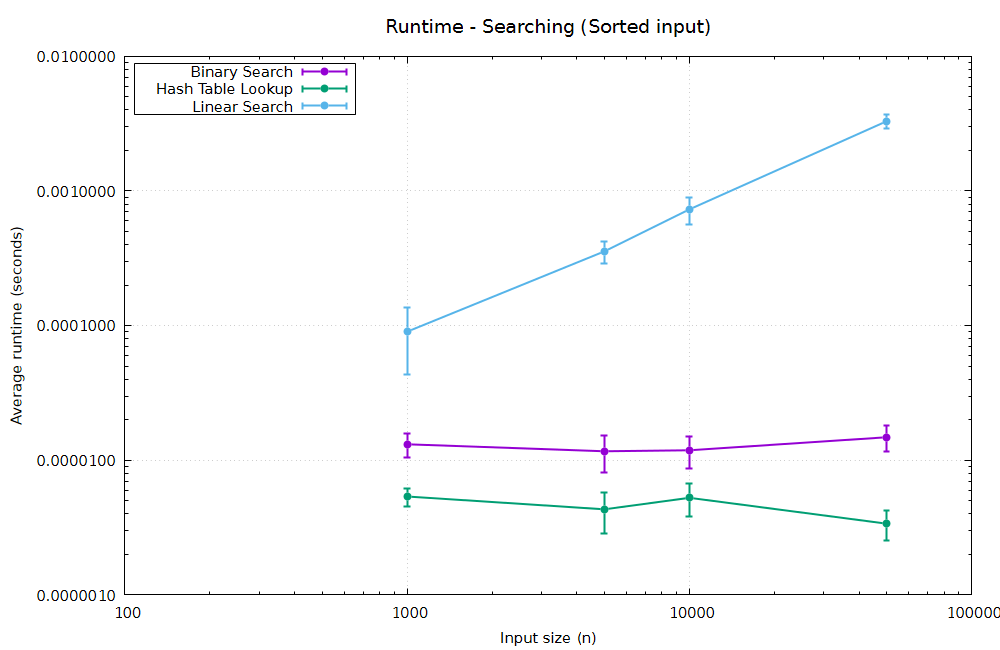
\includegraphics[width=\linewidth,height=0.43\textheight,keepaspectratio]{Searching_Sorted_runtime.png}
      \scriptsize Successful search on sorted arrays, $n=1,000$ to $50,000$.
  \end{columns}
  \vspace{0.4em}
  \begin{block}{Observed at largest tested size}
    At $n=5,000$, Insertion Sort took 0.540 s versus Quick Sort's 0.0128 s.
    At $n=50,000$, Linear Search took 3.296 ms; Binary Search took 0.0148 ms.
  \end{block}
\end{frame}

\begin{frame}{Measured Results: Graph and Dynamic Programming}
  \small
  \begin{columns}[T,onlytextwidth]
    \column{0.50\textwidth}
      \centering\textbf{Sparse graph runtime}
      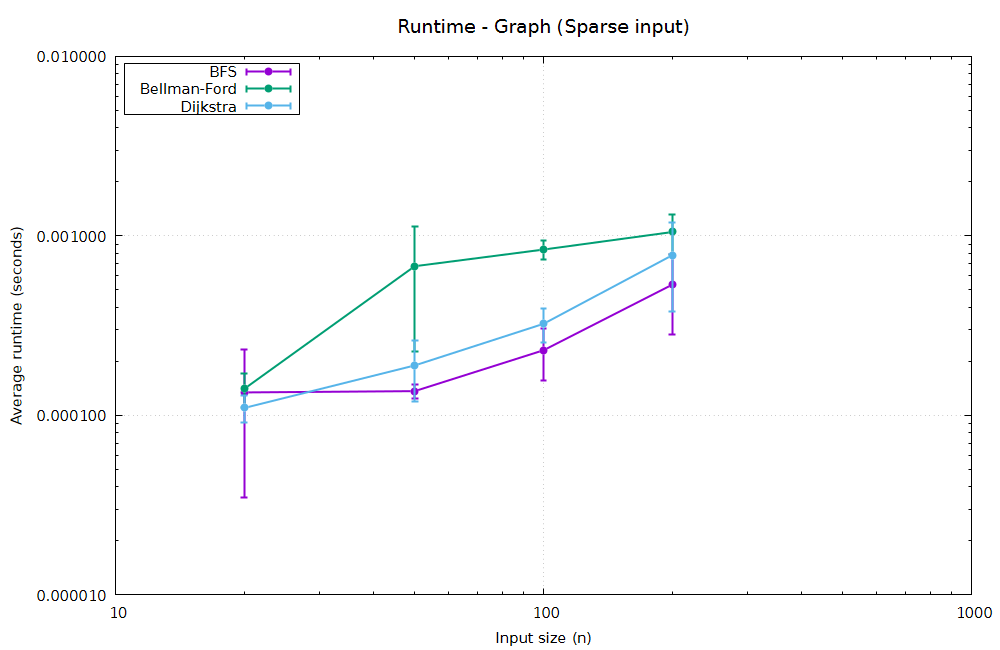
\includegraphics[width=\linewidth,height=0.42\textheight,keepaspectratio]{Graph_Sparse_runtime.png}
      \scriptsize 20--200 vertices.
    \column{0.50\textwidth}
      \centering\textbf{Knapsack runtime}
      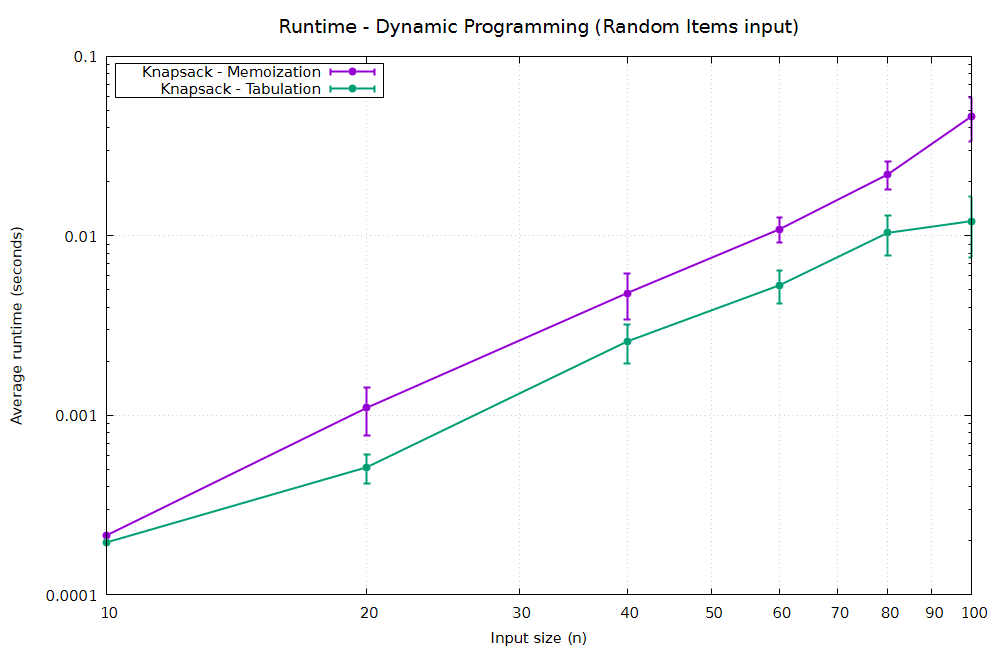
\includegraphics[width=\linewidth,height=0.42\textheight,keepaspectratio]{Dynamic_Programming_Random_Items_runtime.png}
      \scriptsize 10--100 items.
  \end{columns}
  \vspace{0.3em}
  \begin{block}{Observed at largest tested size}
    At 200 vertices, Dijkstra took 0.781 ms and Bellman--Ford 1.051 ms.
    At 100 items, Knapsack tabulation took 12.086 ms versus 46.322 ms for memoization.
  \end{block}
\end{frame}

\begin{frame}{Measured Results: Matrix Multiplication}
  \small
  \begin{columns}[T,onlytextwidth]
    \column{0.50\textwidth}
      {\centering\textbf{Runtime}\par}
      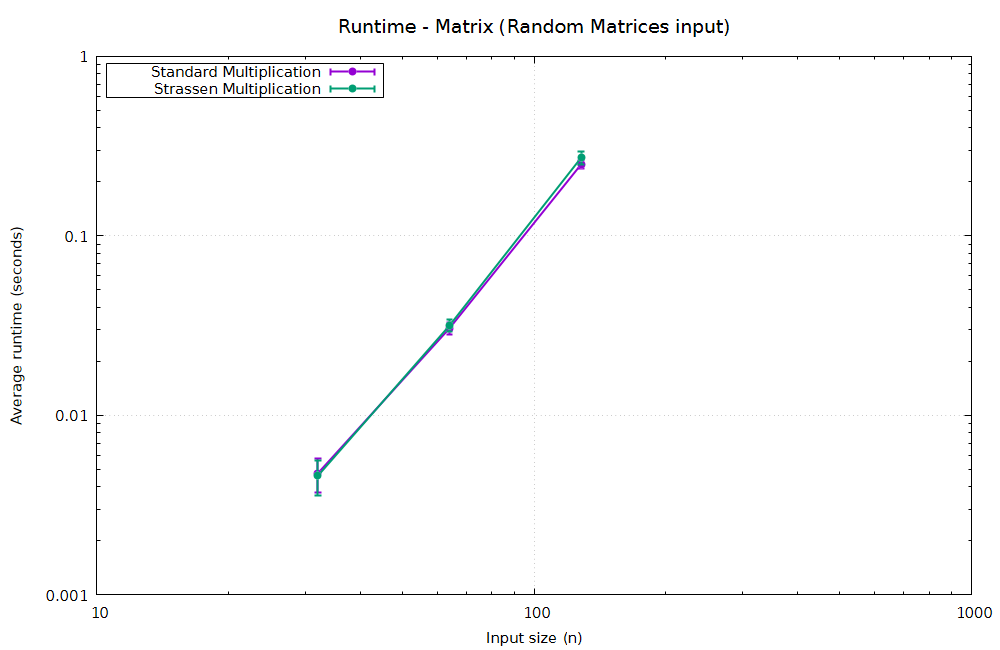
\includegraphics[width=0.98\linewidth,height=0.40\textheight,keepaspectratio]{Matrix_Random_Matrices_runtime.png}
    \column{0.50\textwidth}
      {\centering\textbf{Peak additional memory}\par}
      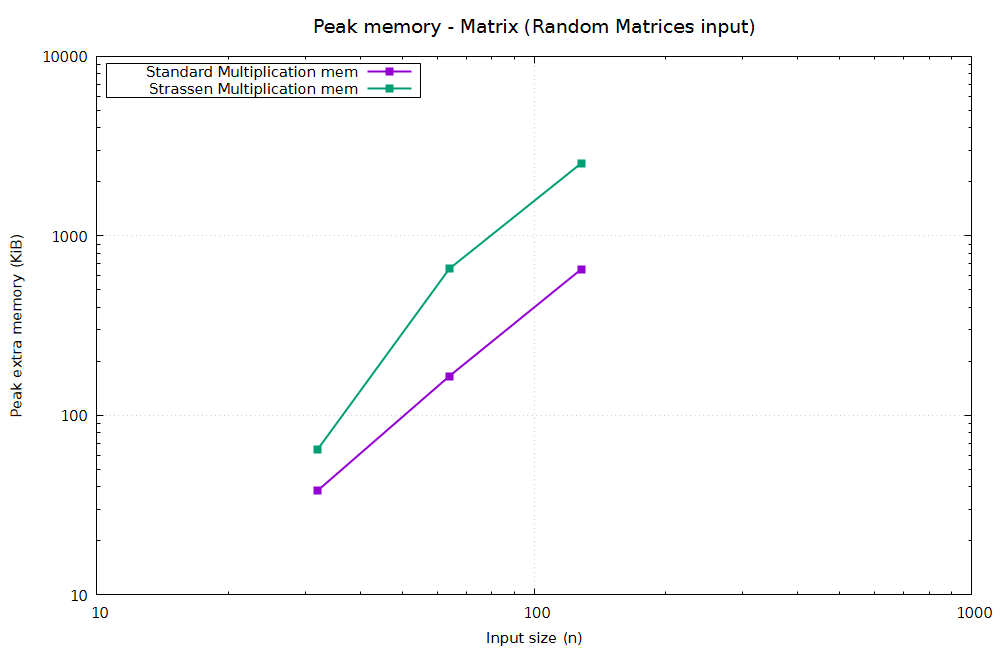
\includegraphics[width=0.98\linewidth,height=0.40\textheight,keepaspectratio]{Matrix_Random_Matrices_memory.png}
  \end{columns}
  \begin{block}{Dimension 128}
    Standard: 249.948 ms and 650.7 KiB. Strassen: 272.290 ms and 2,533.3 KiB.
    The tested sizes did not reach a Strassen runtime crossover.
  \end{block}
\end{frame}

\begin{frame}{Profiler Findings and Interpretation}
  \small
  \begin{itemize}
    \item Quick Sort ($n=5,000$): 5,971 recursive \texttt{sort} calls in the profile.
    \item Knapsack memoization ($n=100$): 45,463 recursive \texttt{solve} calls and 44,869 calls to \texttt{max}.
    \item Strassen ($n=128$): 57 recursive calls, plus repeated matrix add/subtract and base-case multiplication.
  \end{itemize}
  \begin{alertblock}{Measurement caveat}
    Some cProfile captures also include Streamlit watcher and event-loop activity. Their cumulative times are not attributable solely to the algorithm; isolate profiling in a worker process in a future version.
  \end{alertblock}
  \begin{block}{Validation}
    158 pytest cases and 64 subtests passed in the integration test environment; all 16 registered algorithms were smoke-tested through the engine. The local dashboard generated five-category CSV and GNUplot evidence.
  \end{block}
\end{frame}

\begin{frame}{Five-Minute Demonstration}
  \begin{enumerate}
    \item 0:00--0:40 — Problem and AlgoBench overview.
    \item 0:40--1:30 — Select category, algorithms, input distribution, and sizes.
    \item 1:30--2:30 — Run experiment; inspect runtime and memory results.
    \item 2:30--3:20 — Compare scaling and show CSV/GNUplot output.
    \item 3:20--4:15 — Show cProfile bottleneck report.
    \item 4:15--5:00 — Show tests, Bash/Makefile automation, and conclusion.
  \end{enumerate}
\end{frame}

\begin{frame}{Conclusion}
  \begin{itemize}
    \item AlgoBench connects algorithm implementations to a reusable experiment engine.
    \item Reproducible datasets and repeated measurements support meaningful comparisons.
    \item Separate timing, memory, and profiling runs improve measurement clarity.
    \item CSV history and GNUplot provide reproducible evidence for analysis.
  \end{itemize}
  \vfill
  \centering
  \Large Thank you\\[0.4em]
  \normalsize Questions?
\end{frame}

\end{document}
